\setcounter{section}{2}

\Needspace{5\baselineskip}
\hypertarget{context-engineering}{%
\section{Context Engineering}\label{context-engineering}}

\Needspace{5\baselineskip}
\hypertarget{i.-improving-the-cache-hit-rate}{%
\subsection{I. Improving the Cache Hit Rate}\label{i.-improving-the-cache-hit-rate}}

Each iteration of an agent loop resends the previous conversation history, including lengthy error messages and file contents, to the model, causing computational complexity to grow quadratically. Caching strategies can maximize KV cache hits.

From a caching perspective, context is often arranged from front to back as global cache (system instructions and tool definitions), task/project cache (such as CLAUDE.md and AGENT.md), session cache (conversation history), and current session messages (user input, environmental feedback, and so on). Place static content as early as possible and dynamic content toward the end. The server can retrieve the unchanged prefix directly from cached history without recalculating it.

This reduces the cost growth of long conversations from quadratic to linear. However, any change to system instructions, tool definitions, or conversation history invalidates the cache, including switching models midway, changing the working directory, modifying permission configurations, or changing the MCP tool list. Methods for maximizing cache hits include:

\begin{enumerate}
\def\labelenumi{\arabic{enumi}.}
\item
  Keep the prompt prefix stable. Because LLMs are autoregressive, even a single-token difference invalidates the cache after that token. For example, append a message to the input for configuration or tool changes whenever possible; a system prompt change can use something like \texttt{\textless{}system-reminder\textgreater{}} rather than discarding the entire cache. A common mistake is putting a timestamp, especially one precise to the second, at the beginning of the system prompt, greatly reducing the cache hit rate.
\item
  Make session context append-only. Avoid modifying earlier actions or observations. Note that many programming languages and libraries do not guarantee stable key order when serializing JSON objects, which can silently break caching. Whenever possible, compact context when a cache miss would occur anyway.
\item
  Explicitly mark cache breakpoints when needed. Some model providers or inference frameworks do not support automatic incremental prefix caching and instead require manually inserted cache breakpoints. Account for possible cache expiration when placing them and ensure, at minimum, that a breakpoint includes the end of the system prompt.
\end{enumerate}

\begin{figure}[htbp]
\centering
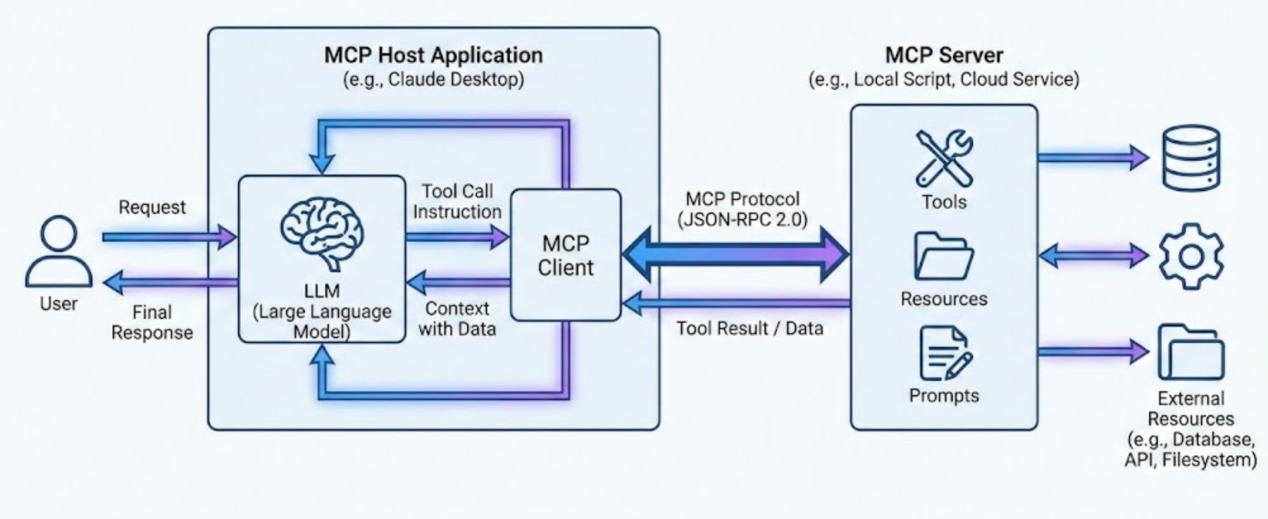
\includegraphics{images/image-0036.png}
\caption{Designing context around the KV cache}
\end{figure}

\Needspace{5\baselineskip}
\hypertarget{ii.-tool-management}{%
\subsection{II. Tool Management}\label{ii.-tool-management}}

As agents become more capable, their action spaces naturally become more complex, with an explosive increase in tool count. If users can define their own tools, someone will inevitably insert hundreds of obscure tools into the action space. The model then becomes more likely to choose the wrong action or an inefficient path, making the agent less intelligent.

A natural response is to design a dynamic action space, loading tools on demand through a RAG-like method and including only the loaded tools in context. However, experiments indicate that dynamically adding or removing tools during iteration should be avoided unless absolutely necessary. Tool definitions occur near the beginning of context, so any change invalidates the KV cache for all subsequent actions and observations. In addition, the model becomes confused when earlier actions and observations refer to tools no longer defined in the current context. Without constrained decoding, this often leads to schema violations or hallucinated actions.

\Needspace{5\baselineskip}
Methods that address this problem while improving action selection include:

\begin{enumerate}
\def\labelenumi{\arabic{enumi}.}
\tightlist
\item
  Keep only ``meta-tools'' in context. Invoking them guides the model to the locations where specific tools are stored in the filesystem. This is also a form of progressive disclosure, making tools flexible and extensible.
\end{enumerate}

For example, Claude Code's \href{https://simonwillison.net/2025/Oct/16/claude-skills/\#skills-depend-on-a-coding-environment}{skills are stored in the filesystem} rather than bound as tools. Claude needs only a few simple functions, such as Bash and filesystem access, to discover and use skills progressively, autonomously extracting the skills it needs. This only accumulates session context without changing the tool definitions at its beginning.

Manus similarly retains fewer than 20 ``atomic functions,'' such as executing Bash commands, reading and writing files, and running Python code. Complex business logic is wrapped in CLIs (command-line programs) in a sandbox, so the model does not need the JSON schemas of hundreds of MCP tools. It only needs to know, ``I can use Bash.'' To use an MCP tool, it enters a command such as mcp-cli run some\_tool directly in the Bash tool. This also requires no retrieval through a semantic-similarity vector index.

\begin{enumerate}
\def\labelenumi{\arabic{enumi}.}
\setcounter{enumi}{1}
\item
  Retain only a lightweight tool list and let the model retrieve and load full definitions when needed. The tool search introduced in the GPT-5.4 API follows this approach: the model first receives a lightweight list of available tools and a tool-search capability. When it needs a tool, it looks up the full definition and appends it to the conversation. This mechanism does not require definitions to be stored in the filesystem; their storage and retrieval depend on the implementation.
\item
  When a tool needs to be removed, keep it in context but mask token logits during decoding to prevent or force particular actions based on the current context. Alternatively, prompt the model not to use particular tools. However, this essentially becomes a contest over attention, and the model still has some probability of ``breaking the rules'' and generating a disabled tool call.
\end{enumerate}

\begin{figure}[htbp]
\centering
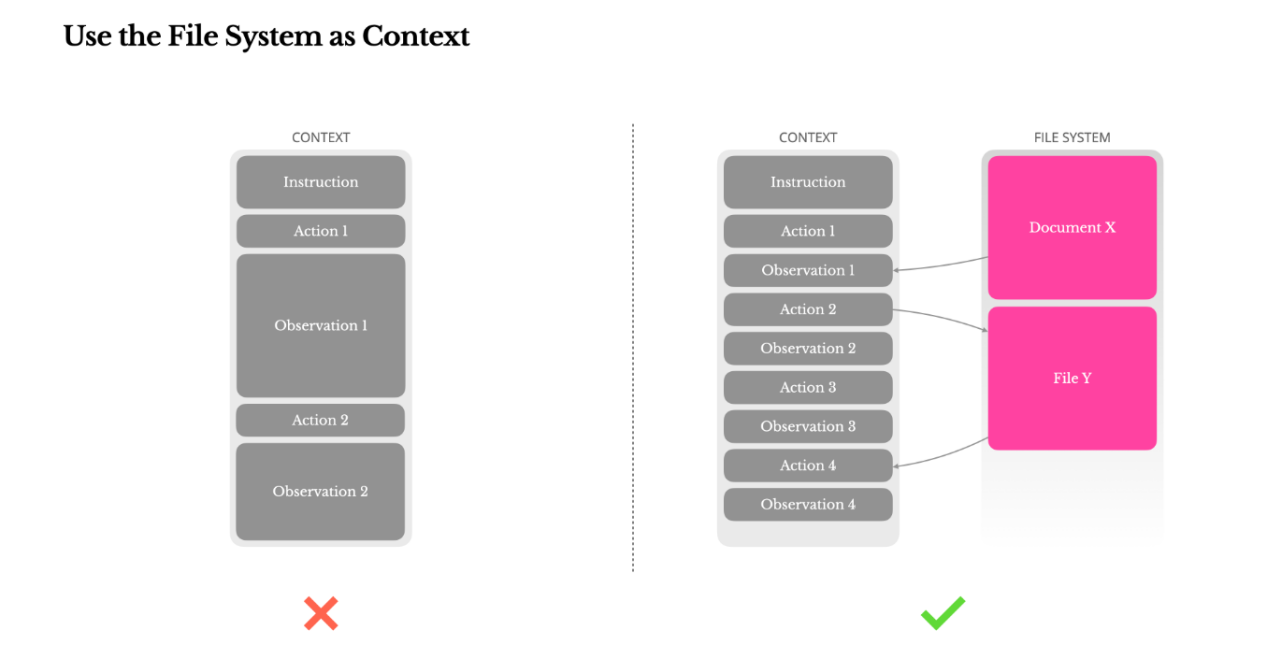
\includegraphics{images/image-0037.png}
\caption{Managing tools by masking rather than removing them}
\end{figure}

\Needspace{5\baselineskip}
Function calling usually has three modes:

Auto: the model can choose whether to call a function. Implemented by prefilling only the response prefix: \textless\textbar im\_start\textbar\textgreater assistant

Required: the model must call a function, but its choice is unrestricted. Implemented by prefilling through the tool-call token: \textless\textbar im\_start\textbar\textgreater assistant\textless tool\_call\textgreater{}

Specified: the model must call a function from a particular subset. Implemented by prefilling through the beginning of the function name: \textless\textbar im\_start\textbar\textgreater assistant\textless tool\_call\textgreater\{``name'': ``browser\_''\}

\Needspace{5\baselineskip}
\hypertarget{iii.-a-context-windowfilesystem-hierarchy}{%
\subsection{III. A Context-Window--Filesystem Hierarchy}\label{iii.-a-context-windowfilesystem-hierarchy}}

The context window is limited, and information compression is irreversible. We can therefore keep only important information in context and store the rest in the filesystem. The model learns to write and read files as needed, using the filesystem not only as storage but as structured external memory.

\begin{figure}[htbp]
\centering
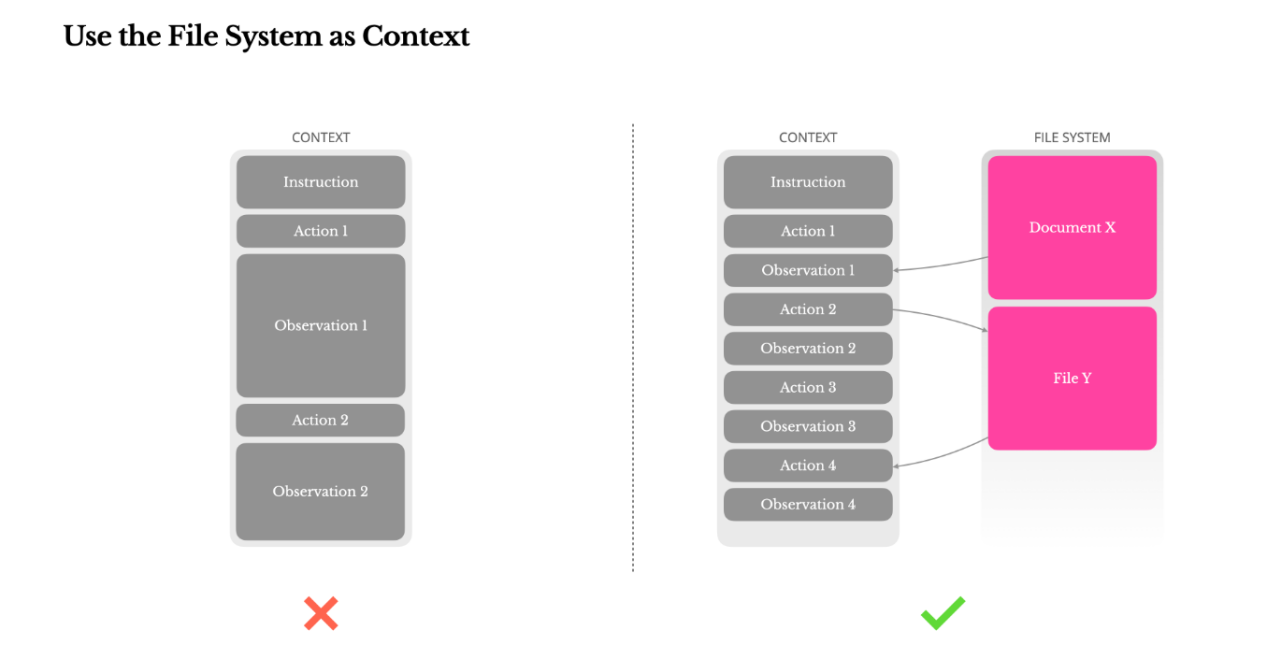
\includegraphics{images/image-0038.png}
\caption{Using the filesystem as context}
\end{figure}

When context is nearly full, the model triggers compaction by appending a message indicating that compaction is needed. Apart from the current conversation round, tool results from previous rounds are compressed into indices pointing to the corresponding content in the filesystem.

\begin{figure}[htbp]
\centering
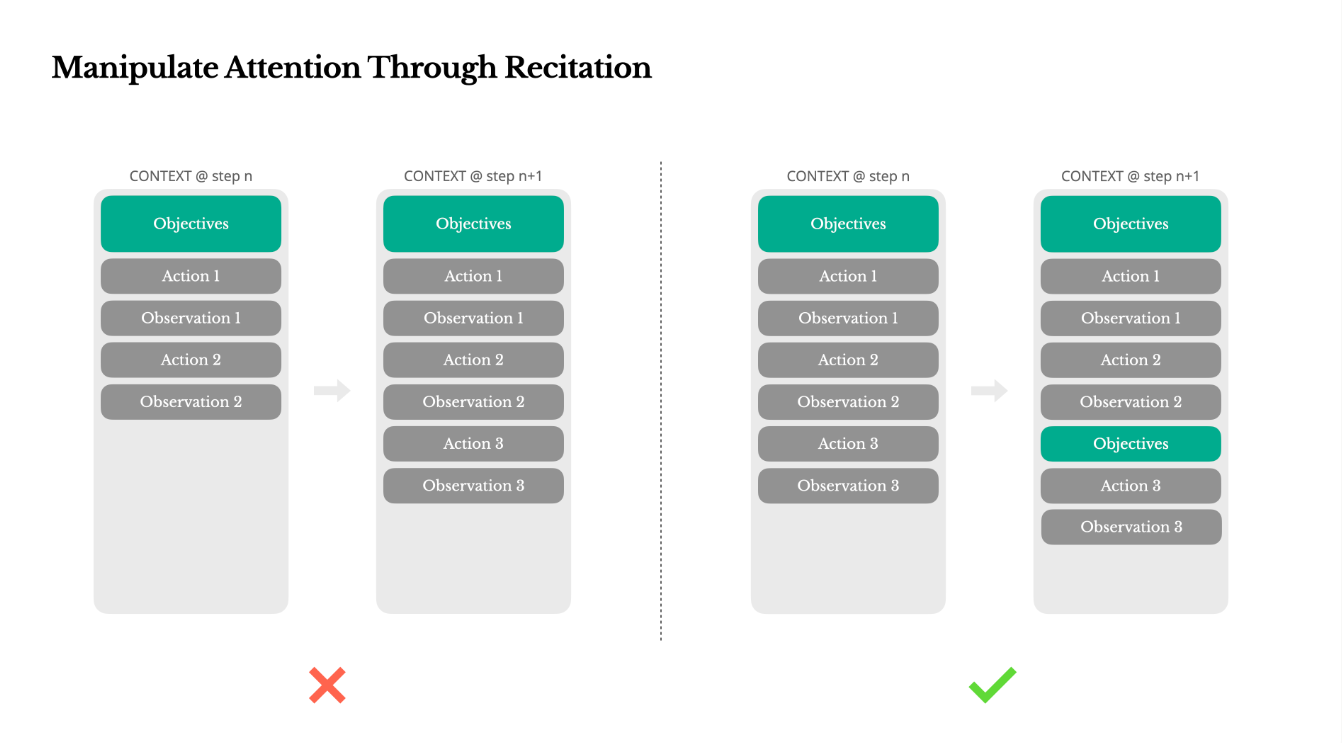
\includegraphics{images/image-0039.png}
\caption{Compacting tool results while retaining necessary content}
\end{figure}

\Needspace{5\baselineskip}
\hypertarget{iv.-restating-objectives}{%
\subsection{IV. Restating Objectives}\label{iv.-restating-objectives}}

For complex tasks, many agents tend to create a plan file such as todo.md and update it as work progresses, checking off completed items. Besides facilitating user review, this more importantly manipulates attention: restating objectives at the end of context prevents the model from drifting away from them in the later stages of a complex task.

\begin{figure}[htbp]
\centering
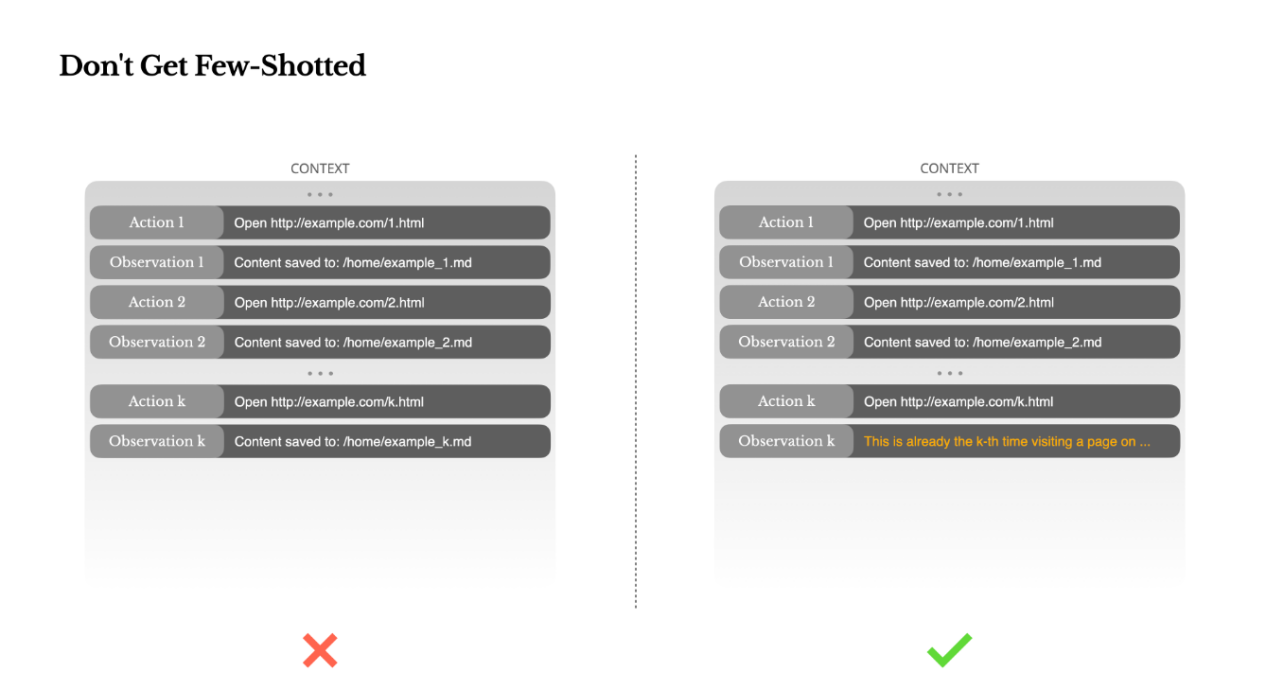
\includegraphics{images/image-0040.png}
\caption{Manipulating attention by restating objectives}
\end{figure}

\Needspace{5\baselineskip}
\hypertarget{v.-avoiding-few-shot-lock-in}{%
\subsection{V. Avoiding Few-Shot Lock-In}\label{v.-avoiding-few-shot-lock-in}}

Language models are excellent imitators: they imitate behavioral patterns in context. If context is filled with similar past action--observation pairs, the model tends to follow that pattern even when it is no longer optimal. This can be dangerous in tasks involving repeated decisions or actions. For example, when reviewing 20 résumés, an agent often falls into a rhythm of repeating similar actions simply because it sees them in context. This leads to drift, overgeneralization, or occasional hallucinations.

The solution is to introduce diversity through small structured variations in actions and observations, such as different serialization templates, alternative wording, or minor noise in ordering or formatting. This controlled randomness helps break patterns and redirect the model's attention.

\begin{figure}[htbp]
\centering
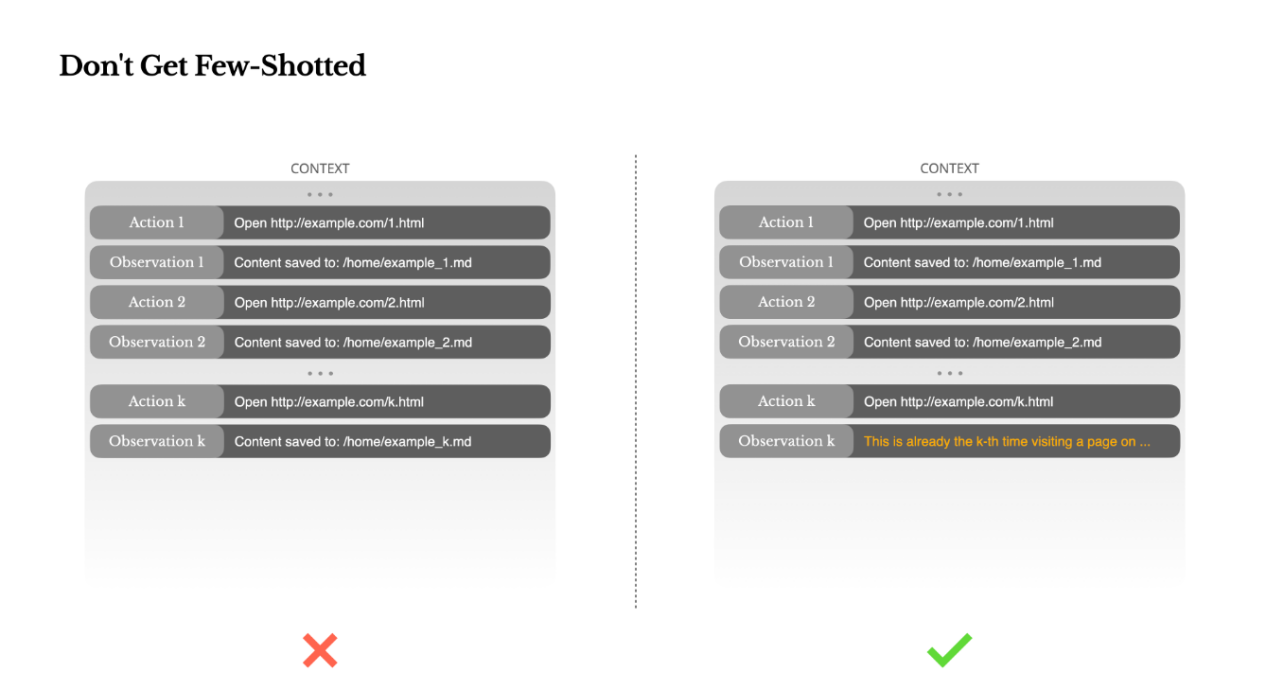
\includegraphics{images/image-0041.png}
\caption{Avoiding behavioral lock-in from few-shot examples}
\end{figure}

\Needspace{5\baselineskip}
\hypertarget{vi.-context-isolation-in-multi-agent-systems}{%
\subsection{VI. Context Isolation in Multi-Agent Systems}\label{vi.-context-isolation-in-multi-agent-systems}}

In a multi-agent system, the main agent and subagents, for example serving as planner and executor, have some context isolation, such as different system prompts and tool definitions. The remaining context need not be shared, although sharing is still recommended for complex tasks with long context.

\Needspace{5\baselineskip}
A nonsharing paradigm:

\begin{figure}[htbp]
\centering
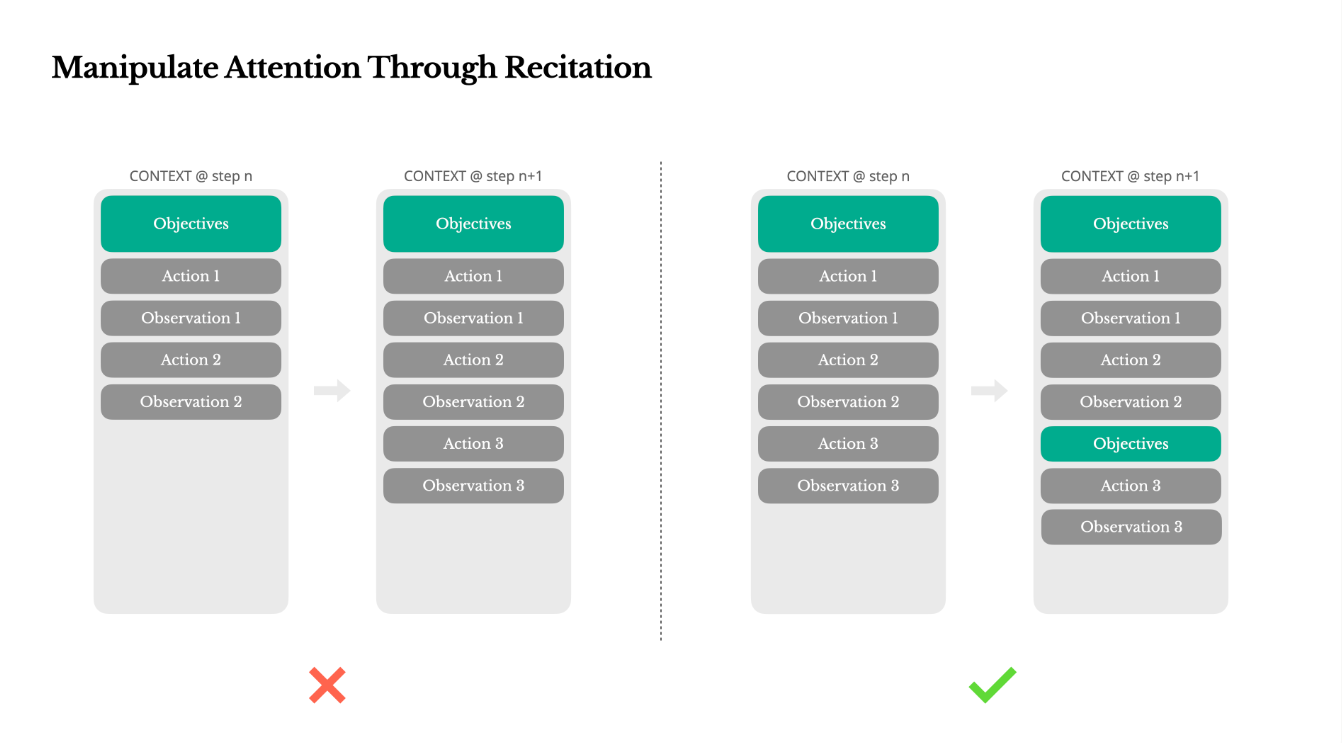
\includegraphics{images/image-0042.png}
\caption{Isolating main-agent and subagent contexts through communication}
\end{figure}

A partially shared paradigm: for example, the main agent acts as planner and shares the full context with subagents. Each subagent retains its own action space (tools) and instructions but receives the full context available to the planner.

\begin{figure}[htbp]
\centering
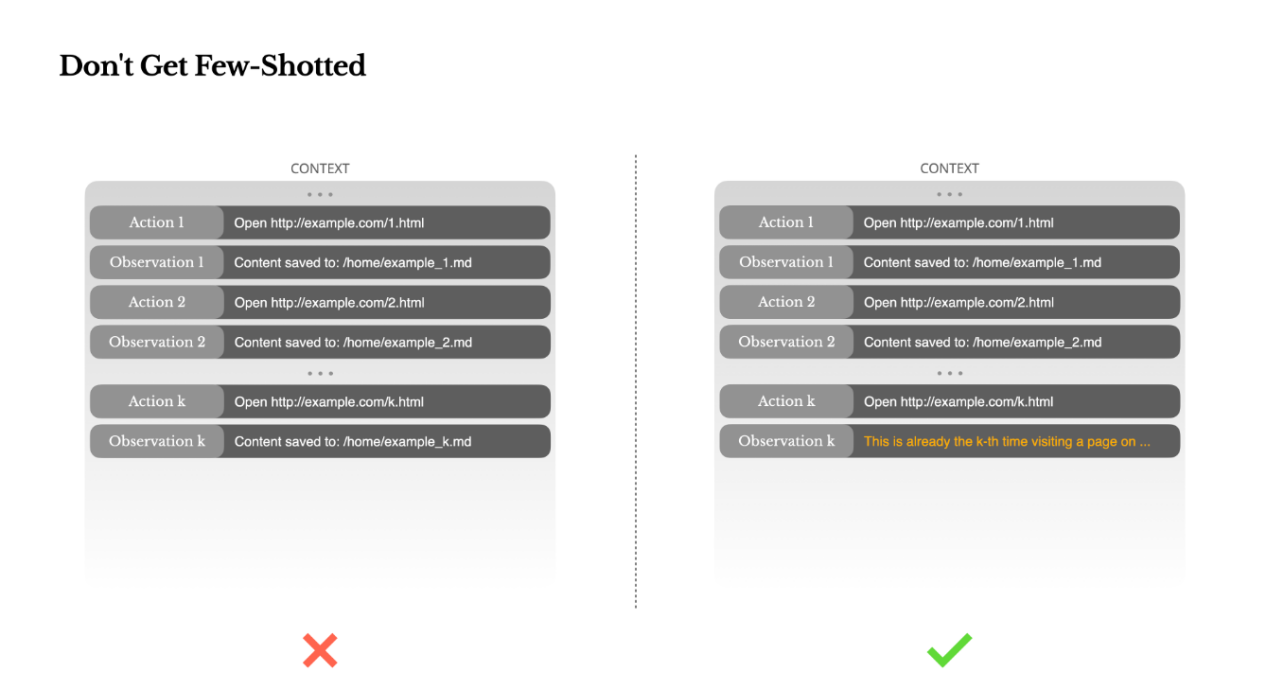
\includegraphics{images/image-0043.png}
\caption{Sharing context between the main agent and subagents}
\end{figure}

\FloatBarrier
\Needspace{5\baselineskip}
\hypertarget{references-127}{%
\subsection{References}\label{references-127}}

\vspace{0.25em}
\begin{itemize}
\tightlist
\item
  Martin, L. (2025). \href{https://rlancemartin.github.io/2025/10/15/manus/}{Context Engineering in Manus}.
\item
  Ji, Y. (2025). \href{https://manus.im/zh-cn/blog/Context-Engineering-for-AI-Agents-Lessons-from-Building-Manus}{Context Engineering for AI Agents: Lessons from Building Manus}. Manus.
\item
  OpenAI. (2026). \href{https://openai.com/index/introducing-gpt-5-4/}{Introducing GPT-5.4}.
\end{itemize}

\clearpage
